\documentclass{article}

\usepackage{pgfplots}

\usepgfplotslibrary{fillbetween}


\begin{document}

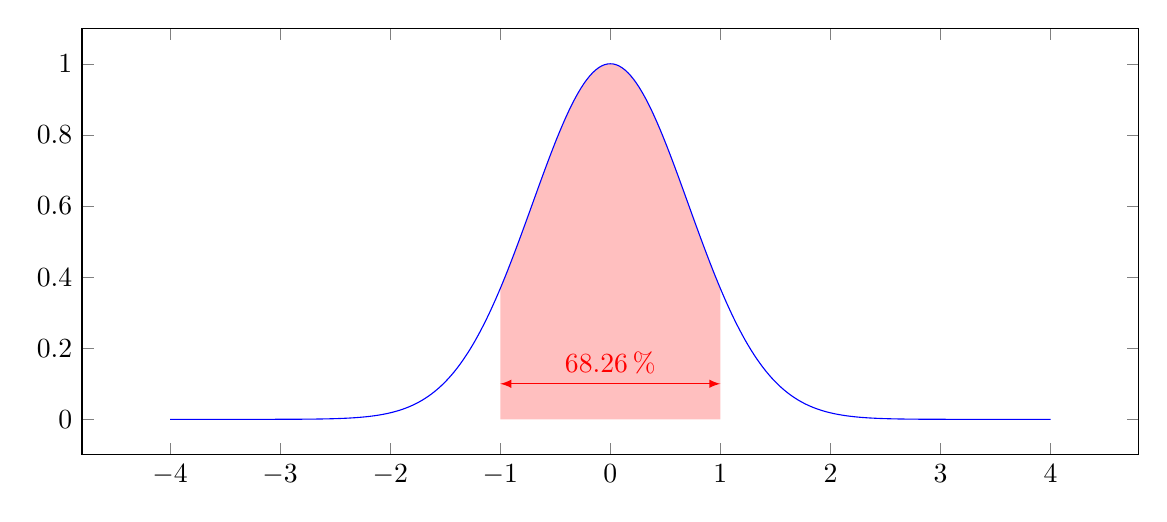
\begin{tikzpicture}

\begin{axis}[
    width=15cm,
    height=7cm]

%% Plot bell curve
\addplot [blue, mark=none, samples=301, name path=f,domain=-4:4] { exp(-x^2) };

%% Just a path over the x axis
\path[name path=xaxis] (axis cs:-4,0) -- (axis cs:4,0);

%% Fill the area between x axis and bell curve, from x = -1 to x = 1 (1 sigma)
\addplot [thick, fill=red, fill opacity=0.25]
              fill between[of=f and xaxis, soft clip={domain=-1:1}];
        
%% Draw the 1 sigma from-to line
\draw[red,latex-latex] (axis cs:-1,0.1) -- (axis cs:1,0.1) node[midway, above] {68.26\,\%};

\end{axis}

\end{tikzpicture}

\end{document}